%!TEX root = ../../main.tex
\subsection{Spin Images}
\frame{
	\frametitle{Spin Images (1999) Johnson \& Herbert}
%	\begin{description}
%		\item[Berechnungsvorschrift] rotiere \textbf{Histogramm} um Referenzachse
%	\end{description}
		\begin{itemize}
		\item Berechne Oberflächennormale im Zielpunkt $\rightarrow$ Referenzachse
		\item Spanne Zylinder $z=(r,h)$ um RA auf
		\item rotiere \textbf{Histogramm} um RA
		\item Zähle Punkte auf ``Umlaufbahn'' $(r,h)$ $\rightarrow$ Spin-Image
		\item Wähle dabei nur Punkte, deren Normale maximal einen gewählten Winkel von der Punktnormale abweicht
	\end{itemize}
	\centering
		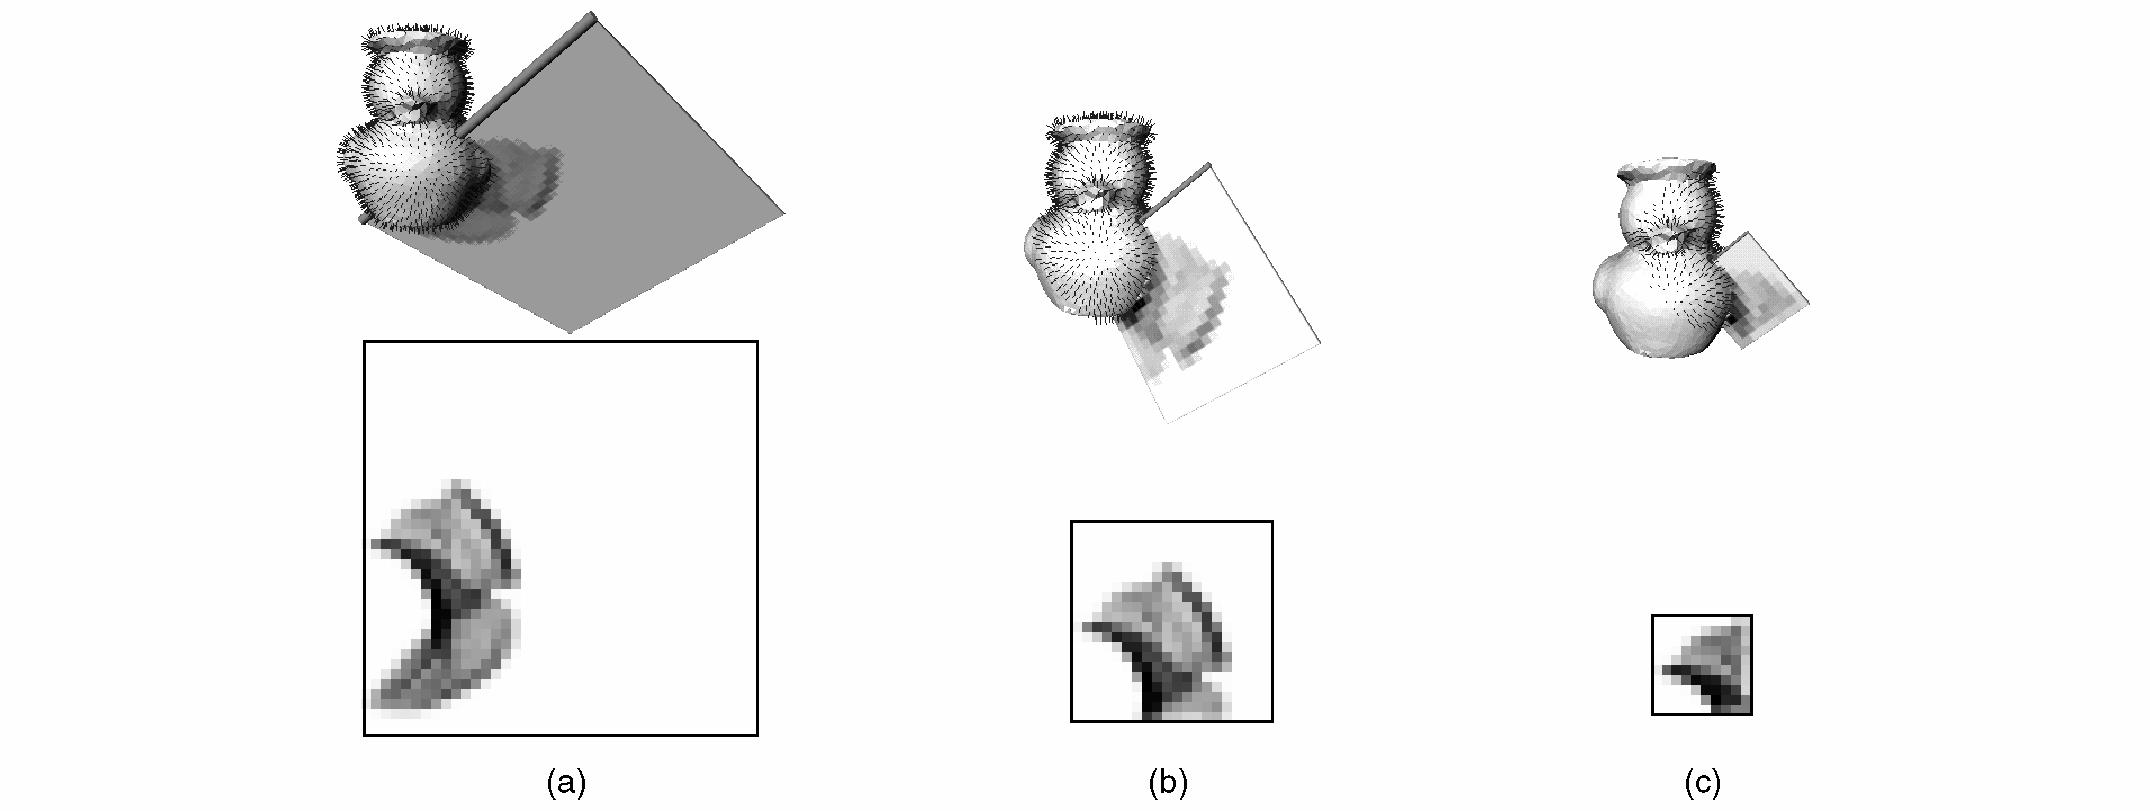
\includegraphics[width=\textwidth]{topics/auswahl/spinImages/si1.jpg}

}

\frame{
	\frametitle{Spin Images (1999) Johnson \& Herbert}
	\begin{flushleft}
	\setbeamertemplate{description item}[align left]
	\begin{description}
		\item[Parameter] Zylinderradius und -höhe, Normalenschwellenwert, Histogrammauflösung
	\item[Referenz] 
		\begin{itemize}
			\item Referenzachse in Punktnormale
			\item Nicht eindeutig aufgrund des Vorzeichens
		\end{itemize}
	\item[Berechnugsmethode] Histogramm
	%\item[Vergleich] Korrelation
    \end{description}
    \end{flushleft}
    \centering
		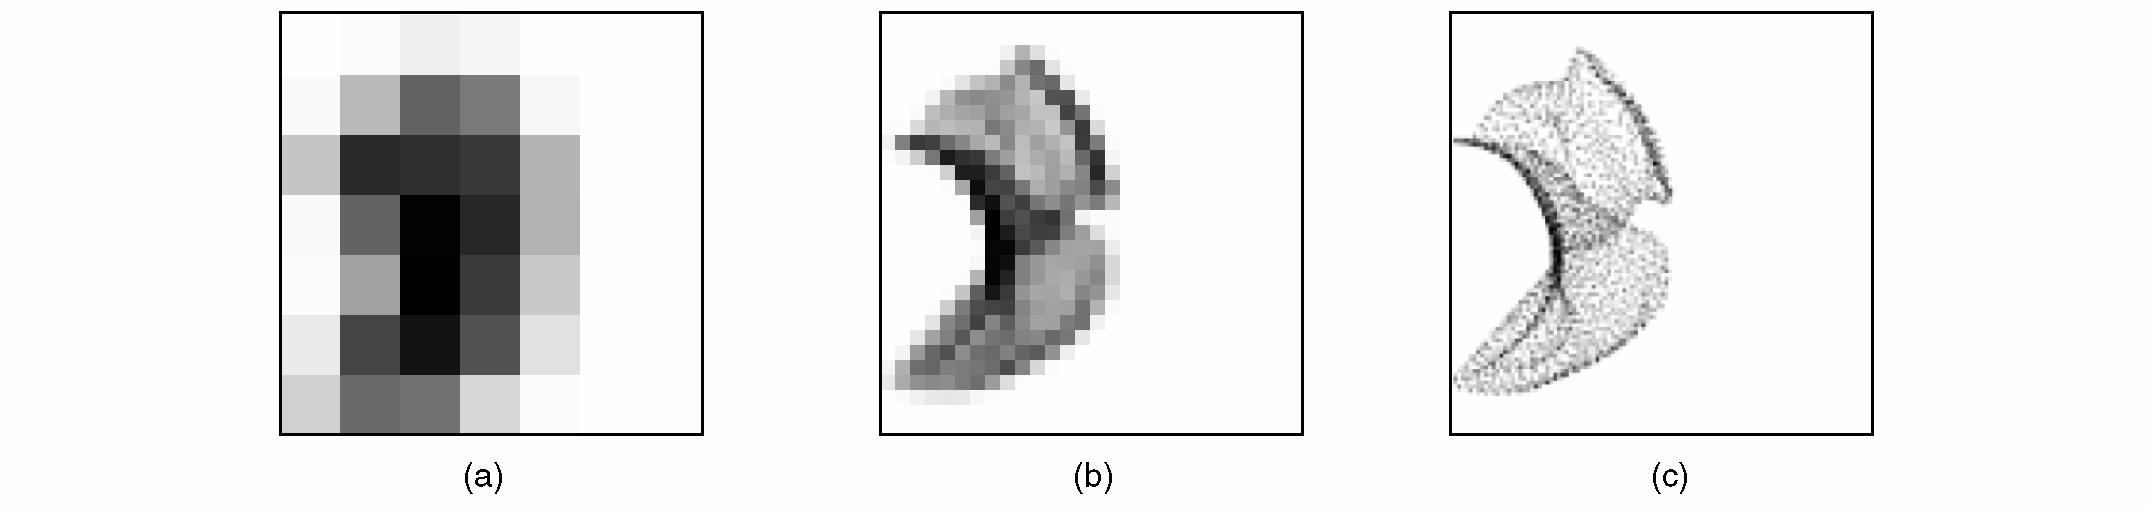
\includegraphics[width=\textwidth]{topics/auswahl/spinImages/si2.jpg}
}	



\subsection{Point Signatures}
\frame{
	\frametitle{Point Signatures (1996)  Chua \& Jarvis}

			\begin{itemize}
		\item Berechne Oberflächennormale im Zielpunkt $p$ $\rightarrow$ $N$
		\item Lege Sphäre mit Radius $r$ um $p$
		\item Schneide Sphäre mit Oberfläche $\rightarrow$ 3D-Kurve $C$
		\item Approximiere tangentiale Ebene an $p$ $\rightarrow$ $P'$
		\item Projiziere $C$ auf $P'$  $\rightarrow$ planare Kurve $C'$
		\item Wähle Referenzwinkel $\Theta_0$ nach dem höchsten Wert in $C'$

	\end{itemize}

	\centering
		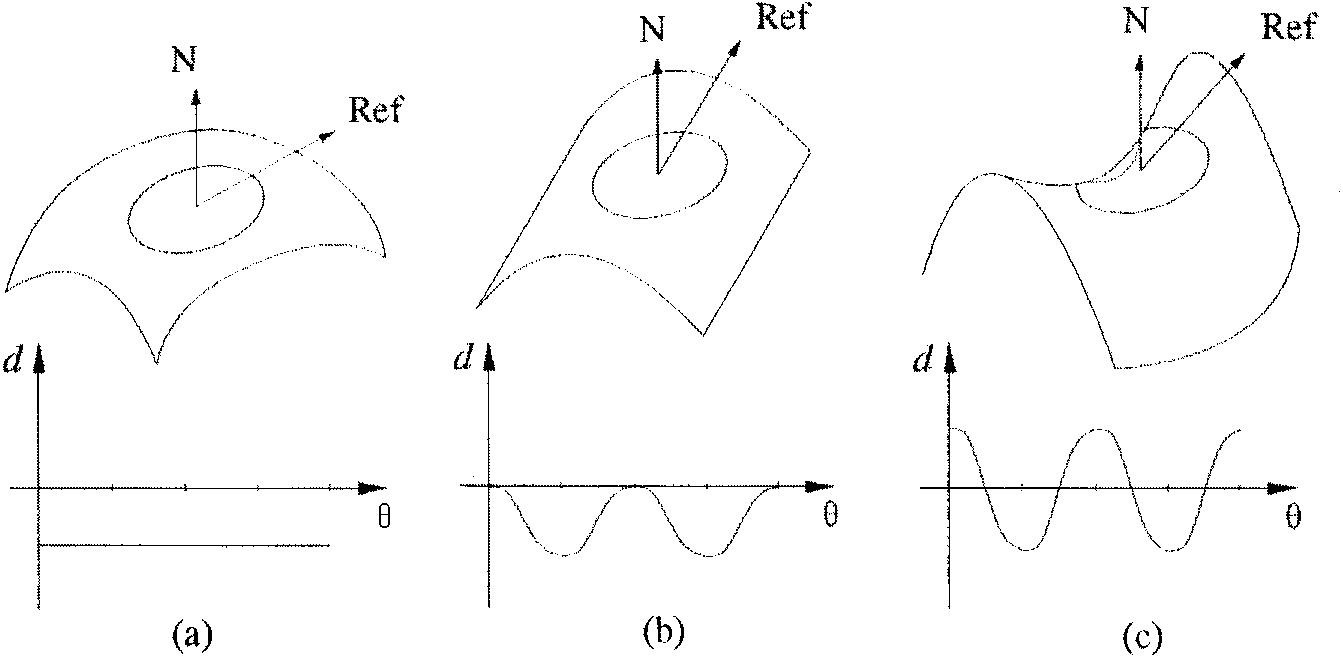
\includegraphics[width=0.8\textwidth]{topics/auswahl/pointSignatures/ps.jpg}
}

\frame{
	\frametitle{Point Signatures (1996)  Chua \& Jarvis}
	\begin{flushleft}
	\setbeamertemplate{description item}[align left]
	\begin{description}
		\item[Parameter] Sphärenradius, Schwellenwert
	\item[Referenz] 
		\begin{itemize}
			\item Referenzrahmen, Normale und Startwinkel, Anzahl der Skalen
			\item Variant gegenüber Skalierung, da fester Radius $\rightarrow$ berechne mit mehreren Radien pro Modell
		\end{itemize}
	\item[Berechnugsmethode] Signatur
	\item[Vergleich] $|d_1(\Theta_i)-d_2(\Theta_i) > \epsilon|$


    \end{description}
    \end{flushleft}

    \centering
		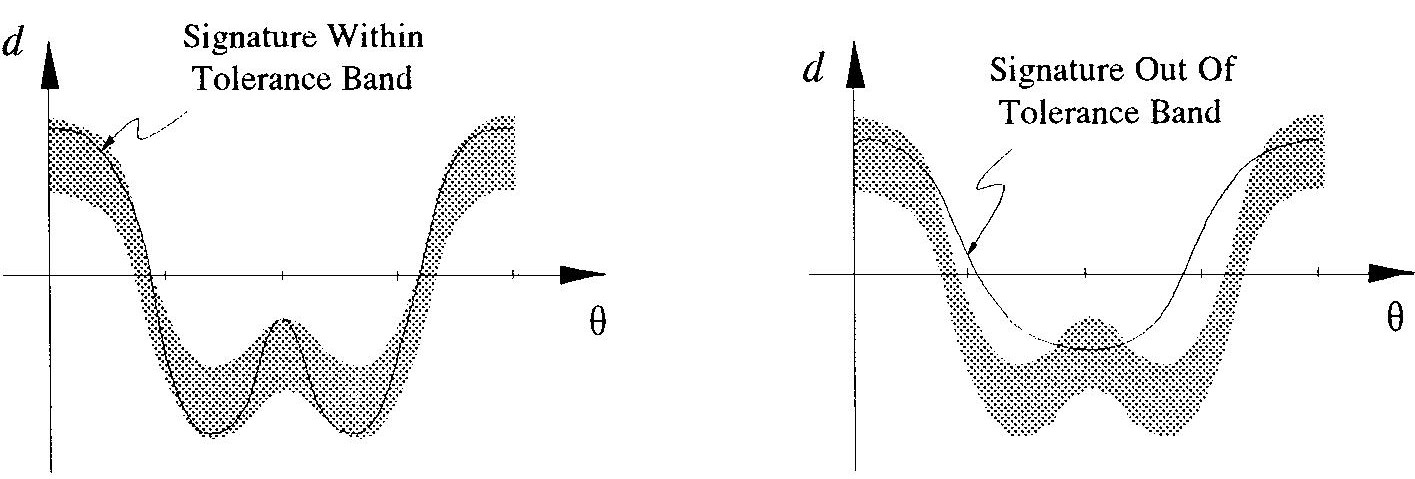
\includegraphics[width=0.8\textwidth]{topics/auswahl/pointSignatures/m.jpg}
}




\subsection{Exponential Mapping}
\frame{
	\frametitle{Exponential Mapping (2008) Novatnack \& Nishino}

			\begin{itemize}
		\item Wähle eine sphärische Nachbarschaft mit Radius $\sigma$ für den Zielpunkt $p$
		\item Berechne für jeden Nachbarn die geodätischen Koordinaten $\mathbb{G}(u,v)=(d_g(u,v),\Theta_\tau(u,v))$
		\item Fasse die für jeden Nachbarn berechneten Tupel als skalenabhänigen Deskriptor $\mathbb{G}^\sigma_p$ zusammen.
		\item Berechne $\mathbb{G}^\sigma_p$ für mehrere $\sigma$ pro Punkt um skalenunabhängigen Deskriptor zu erzeugen.


	\end{itemize}

    \centering
		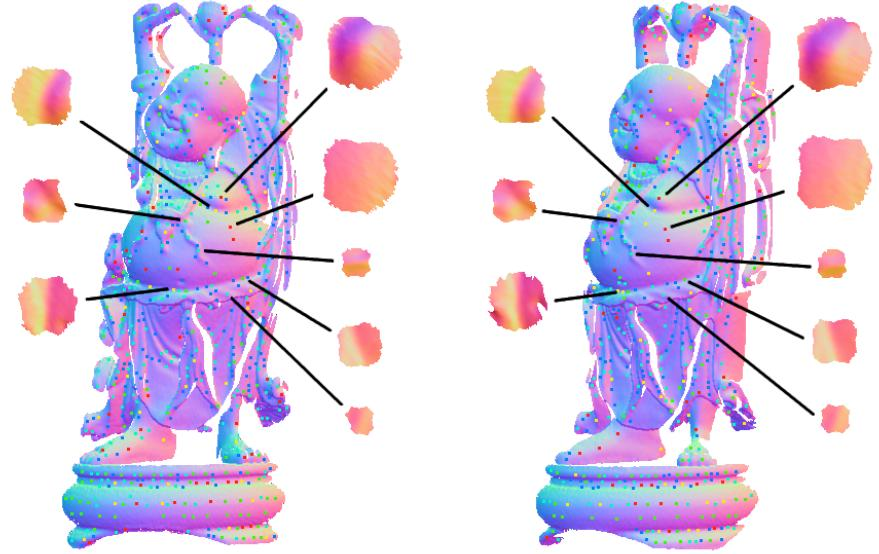
\includegraphics[width=0.4\textwidth]{topics/auswahl/exponentialMapping/em1.jpg}
}

\subsection{Exponential Mapping}
\frame{
	\frametitle{Exponential Mapping (2008) Novatnack \& Nishino}

	\begin{flushleft}
	\setbeamertemplate{description item}[align left]
	\begin{description}
		\item[Parameter] Anzahl der Skalen, Sphärenradien
	\item[Referenz] 
		\begin{itemize}
			\item Referenzrahmen
			\item Variant gegenüber Skalierung, da fester Radius $\rightarrow$ berechne mit mehreren Radien pro Modell
		\end{itemize}
	\item[Berechnugsmethode] Signatur
	%\item[Vergleich] Normalisierte Kreuzkorrelation
\end{description}
    \end{flushleft}

        \centering
		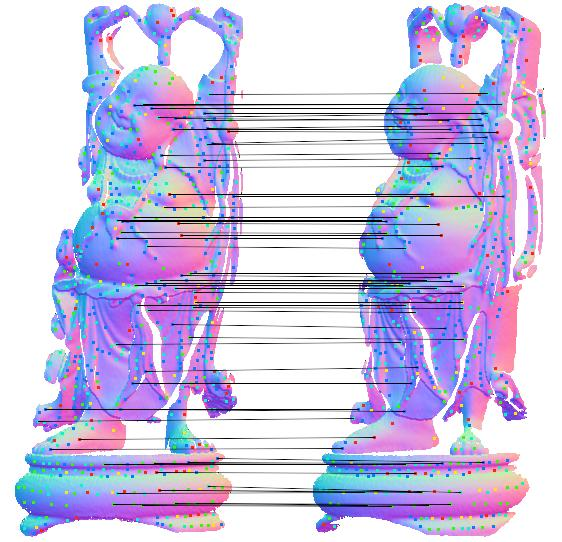
\includegraphics[width=0.4\textwidth]{topics/auswahl/exponentialMapping/em2.jpg}
}

\subsection{SHOT}
\frame{
	\frametitle{Signatures of Histogramms of Orientations}
		\begin{itemize}
		\item Wähle eine sphärische Nachbarschaft mit Radius $R$ für den Zielpunkt $p$ $\rightarrow$ Menge von Nachbarn $p_i$
		\item Berechne Hauptachsen der Matrix $M$ als Referenzsystem via EVD
		\item $M=\frac{1}{\Sigma_{i:d_i \geq R}} \Sigma_{i:d_i \geq R} (R-||p_i-i||_2)(p_i-p)(p_i-p)^T$
		\item Wähle als Achsen $x,y,z$ die Eigenvektoren zu den ersten drei, der absteigend geordneten Eigenwerte
		\item Wähle Vorzeichen der Achsen nach: 
		%\setbeamertemplate{description item}[align left]
		\begin{description}
			\item[$S_x^+$] $=\{i:d \geq R \land (p_i -p) * x^+ \geq 0 \}$
			\item[$S_x^-$] $=\{i:d \geq R \land (p_i -p) * x^- \geq 0 \}$
			\item[x]  = $	\left \{
  							\begin{aligned}
    							&x^+, && \text{wenn}\ |S_x^+| \geq S_x^- \\
    							&x^-, && \text{sonst}
  							\end{aligned} \right.$
		\end{description}
		\item Wähle Vorzeichen für $z$ analog und ermittle $y = z \times x$
	\end{itemize}

	
}

\frame{
	\frametitle{SHOT (2010) Tombari, Salti \& Stefano}
	\setbeamertemplate{description item}[align left]
	\begin{description}
		\item [Idee] \begin{itemize} 
						\item Unterteile Nachbarschaft in Bereiche in sphärischem Koordinatensystem
						\item Bilde Histogramm über die auftretenden Winkel zwischen Normalen aller Punkte pro Bereich
						\item Vereine alle Histogramme zu einem Deskriptor 
					\end{itemize}

		\item[Aufteilung] durch radiale Distanz $r$, polaren Winkel $\Theta$ und Azimuthwinkel $\Phi$


			    \begin{figure}
        \centering
        \begin{subfigure}[b]{0.35\textwidth}
            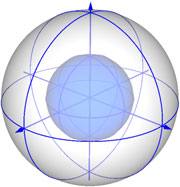
\includegraphics[width=0.8\textwidth]{pdfPics/sphere.png}
            \caption{Sphärisches Koordinatensystem}
            \label{fig:sp}
        \end{subfigure}
        ~~~
        \begin{subfigure}[b]{0.35\textwidth}
            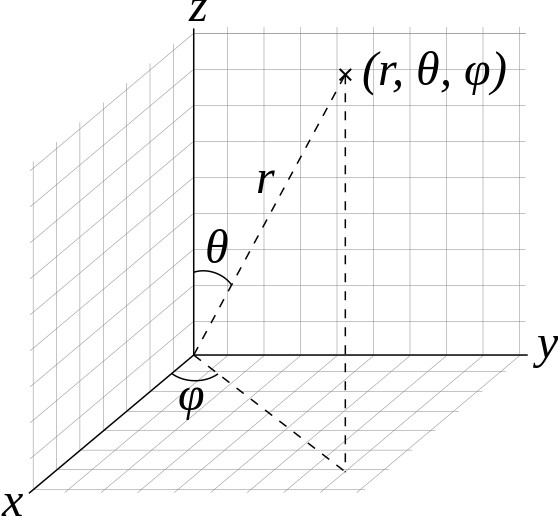
\includegraphics[width=0.8\textwidth]{topics/auswahl/shot/sp.jpg}
            \caption{Benennung}
            \label{fig:Achsen}
        \end{subfigure}
    \end{figure}
	\end{description}
}


\frame{
	\frametitle{SHOT (2010) Tombari, Salti \& Stefano}

	\begin{flushleft}
	\setbeamertemplate{description item}[align left]
	\begin{description}
		\item[Parameter] Anzahl der Auteilungen $(r,\Theta,\Phi)$ für das sphärische Koordinatensystem, Anzahl der Klassen für Winkel zwischen Punktnormalen
	\item[Referenz] 
		\begin{itemize}
			\item Referenzrahmen und Referenzachse
			\item Variant gegenüber Skalierung, da fester Radius $\rightarrow$ berechne mit mehreren Radien pro Modell
		\end{itemize}
	\item[Berechnugsmethode] Signatur von Histogrammen
	%\item[Vergleich] Normalisierte Kreuzkorrelation
\end{description}
    \end{flushleft}

        %\centering
		%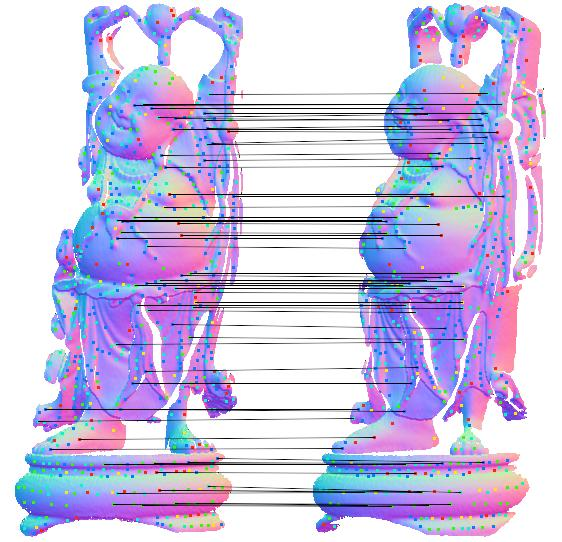
\includegraphics[width=0.4\textwidth]{topics/auswahl/exponentialMapping/em2.jpg}
}